\documentclass[11pt,letterpaper]{article}

% =============================================================================
% PACKAGES
% =============================================================================
\usepackage[margin=1in]{geometry}
\usepackage{enumitem}
\usepackage{setspace}
\usepackage{graphicx}
\usepackage{xcolor}
\usepackage{tikz}
\usetikzlibrary{shapes.geometric, arrows.meta, positioning, fit, backgrounds, calc, decorations.pathreplacing, trees, matrix, shapes.multipart, shapes.symbols, shadows}
\usepackage{tcolorbox}
\usepackage{booktabs}
\usepackage{longtable}
\usepackage{array}
\usepackage{tabularx}
\usepackage{multirow}
\usepackage{colortbl}
\usepackage{fancyhdr}
\usepackage{titlesec}
\usepackage[colorlinks=true,linkcolor=blue!60!black,urlcolor=blue!60!black,citecolor=blue!60!black]{hyperref}
\usepackage{bookmark}
\usepackage{parskip}
\usepackage{float}
\usepackage{caption}
\usepackage{subcaption}
\usepackage{listings}
\usepackage{textcomp}
\usepackage{amssymb}
\usepackage{amsmath}
\usepackage{pifont}

% =============================================================================
% CONFIGURATION
% =============================================================================
\setstretch{1.15}

% Define colors
\definecolor{primary}{RGB}{50, 100, 150}
\definecolor{secondary}{RGB}{80, 130, 180}
\definecolor{accent}{RGB}{200, 100, 50}
\definecolor{success}{RGB}{50, 140, 80}
\definecolor{warning}{RGB}{220, 170, 50}
\definecolor{critical}{RGB}{190, 60, 60}
\definecolor{lightgray}{RGB}{245, 245, 245}
\definecolor{darkgray}{RGB}{80, 80, 80}
\definecolor{patterncolor}{RGB}{230, 240, 255}
\definecolor{principlecolor}{RGB}{255, 245, 230}
\definecolor{decisioncolor}{RGB}{240, 255, 240}
\definecolor{interfacecolor}{RGB}{255, 240, 245}
\definecolor{constraintcolor}{RGB}{250, 245, 255}
\definecolor{codecolor}{RGB}{245, 245, 250}
\definecolor{classcolor}{RGB}{255, 255, 220}

% Section formatting
\titleformat{\section}{\Large\bfseries\color{primary}}{\thesection}{1em}{}[\titlerule]
\titleformat{\subsection}{\large\bfseries\color{secondary}}{\thesubsection}{1em}{}
\titleformat{\subsubsection}{\normalsize\bfseries\color{darkgray}}{\thesubsubsection}{1em}{}

% Header/Footer
\pagestyle{fancy}
\fancyhf{}
\fancyhead[L]{\small\textcolor{darkgray}{Designer's View Specification}}
\fancyhead[R]{\small\textcolor{darkgray}{Architecture Documentation}}
\fancyfoot[C]{\thepage}
\renewcommand{\headrulewidth}{0.4pt}

% Custom environments
\newtcolorbox{definitionbox}[1][]{
    colback=lightgray,
    colframe=primary,
    fonttitle=\bfseries,
    title=#1,
    boxrule=0.5pt,
    arc=2pt,
    left=8pt,
    right=8pt,
    top=6pt,
    bottom=6pt
}

\newtcolorbox{examplebox}[1][]{
    colback=white,
    colframe=secondary,
    fonttitle=\bfseries,
    title=#1,
    boxrule=0.5pt,
    arc=2pt,
    left=8pt,
    right=8pt,
    top=6pt,
    bottom=6pt
}

\newtcolorbox{warningbox}[1][]{
    colback=orange!5,
    colframe=accent,
    fonttitle=\bfseries,
    title=#1,
    boxrule=0.5pt,
    arc=2pt,
    left=8pt,
    right=8pt,
    top=6pt,
    bottom=6pt
}

\newtcolorbox{guidancebox}[1][]{
    colback=green!5,
    colframe=success,
    fonttitle=\bfseries,
    title=#1,
    boxrule=0.5pt,
    arc=2pt,
    left=8pt,
    right=8pt,
    top=6pt,
    bottom=6pt
}

\newtcolorbox{patternbox}[1][]{
    colback=blue!3,
    colframe=primary!70,
    fonttitle=\bfseries,
    title=#1,
    boxrule=0.5pt,
    arc=2pt,
    left=8pt,
    right=8pt,
    top=6pt,
    bottom=6pt
}

\newtcolorbox{principlebox}[1][]{
    colback=orange!5,
    colframe=accent!80,
    fonttitle=\bfseries,
    title=#1,
    boxrule=0.5pt,
    arc=2pt,
    left=8pt,
    right=8pt,
    top=6pt,
    bottom=6pt
}

\newtcolorbox{decisionbox}[1][]{
    colback=green!5,
    colframe=success!80,
    fonttitle=\bfseries,
    title=#1,
    boxrule=0.5pt,
    arc=2pt,
    left=8pt,
    right=8pt,
    top=6pt,
    bottom=6pt
}

\newtcolorbox{constraintbox}[1][]{
    colback=purple!5,
    colframe=primary!60!black,
    fonttitle=\bfseries,
    title=#1,
    boxrule=0.5pt,
    arc=2pt,
    left=8pt,
    right=8pt,
    top=6pt,
    bottom=6pt
}

% Listings configuration
\lstset{
    basicstyle=\ttfamily\small,
    backgroundcolor=\color{codecolor},
    frame=single,
    framerule=0.5pt,
    rulecolor=\color{darkgray},
    breaklines=true,
    captionpos=b,
    tabsize=2,
    showstringspaces=false,
    numbers=left,
    numberstyle=\tiny\color{darkgray},
    numbersep=5pt,
    xleftmargin=15pt,
    keywordstyle=\color{primary}\bfseries,
    commentstyle=\color{darkgray}\itshape,
    stringstyle=\color{success},
    morekeywords={interface, class, abstract, implements, extends, public, private, protected, async, await, const, let, function, return, if, else, for, while, new, this, static, readonly, export, import}
}

% Table column types
\newcolumntype{L}[1]{>{\raggedright\arraybackslash}p{#1}}
\newcolumntype{C}[1]{>{\centering\arraybackslash}p{#1}}
\newcolumntype{R}[1]{>{\raggedleft\arraybackslash}p{#1}}

% Custom commands
\newcommand{\cmark}{\ding{51}}
\newcommand{\xmark}{\ding{55}}

% =============================================================================
% DOCUMENT BEGIN
% =============================================================================
\begin{document}

% -----------------------------------------------------------------------------
% TITLE PAGE
% -----------------------------------------------------------------------------
% Avoid duplicate page anchors caused by titlepage resetting the page counter
\hypersetup{pageanchor=false}
\begin{titlepage}
    \centering
    \vspace*{1.5cm}
    
    {\Huge\bfseries\color{primary} Designer's View\par}
    \vspace{0.5cm}
    {\Large\color{secondary} Architecture Viewpoint Specification\par}
    \vspace{0.3cm}
    {\large\color{darkgray} Design Patterns, Principles, Decisions \& Implementation Guidance\par}
    
    \vspace{1.2cm}
    
    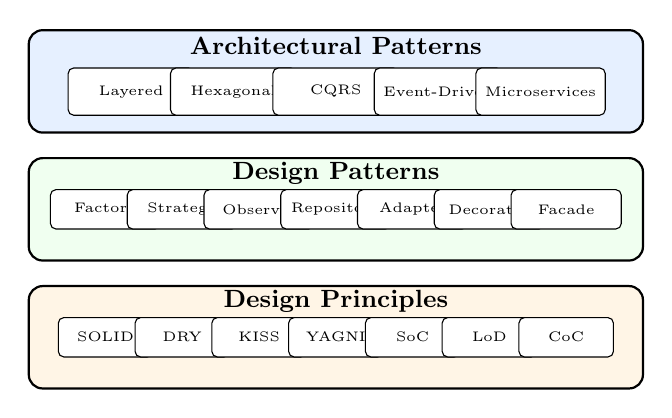
\begin{tikzpicture}[scale=0.65]
        % Design layers
        \draw[thick, fill=patterncolor, rounded corners=5pt] (-6, 2.5) rectangle (6, 0.5);
        \node[font=\small\bfseries] at (0, 2.2) {Architectural Patterns};
        
        \node[draw, fill=white, rounded corners=2pt, minimum width=1.6cm, minimum height=0.6cm, font=\tiny] at (-4, 1.3) {Layered};
        \node[draw, fill=white, rounded corners=2pt, minimum width=1.6cm, minimum height=0.6cm, font=\tiny] at (-2, 1.3) {Hexagonal};
        \node[draw, fill=white, rounded corners=2pt, minimum width=1.6cm, minimum height=0.6cm, font=\tiny] at (0, 1.3) {CQRS};
        \node[draw, fill=white, rounded corners=2pt, minimum width=1.6cm, minimum height=0.6cm, font=\tiny] at (2, 1.3) {Event-Driven};
        \node[draw, fill=white, rounded corners=2pt, minimum width=1.6cm, minimum height=0.6cm, font=\tiny] at (4, 1.3) {Microservices};
        
        % Design patterns
        \draw[thick, fill=decisioncolor, rounded corners=5pt] (-6, 0) rectangle (6, -2);
        \node[font=\small\bfseries] at (0, -0.3) {Design Patterns};
        
        \node[draw, fill=white, rounded corners=2pt, minimum width=1.4cm, minimum height=0.5cm, font=\tiny] at (-4.5, -1) {Factory};
        \node[draw, fill=white, rounded corners=2pt, minimum width=1.4cm, minimum height=0.5cm, font=\tiny] at (-3, -1) {Strategy};
        \node[draw, fill=white, rounded corners=2pt, minimum width=1.4cm, minimum height=0.5cm, font=\tiny] at (-1.5, -1) {Observer};
        \node[draw, fill=white, rounded corners=2pt, minimum width=1.4cm, minimum height=0.5cm, font=\tiny] at (0, -1) {Repository};
        \node[draw, fill=white, rounded corners=2pt, minimum width=1.4cm, minimum height=0.5cm, font=\tiny] at (1.5, -1) {Adapter};
        \node[draw, fill=white, rounded corners=2pt, minimum width=1.4cm, minimum height=0.5cm, font=\tiny] at (3, -1) {Decorator};
        \node[draw, fill=white, rounded corners=2pt, minimum width=1.4cm, minimum height=0.5cm, font=\tiny] at (4.5, -1) {Facade};
        
        % Principles
        \draw[thick, fill=principlecolor, rounded corners=5pt] (-6, -2.5) rectangle (6, -4.5);
        \node[font=\small\bfseries] at (0, -2.8) {Design Principles};
        
        \node[draw, fill=white, rounded corners=2pt, minimum width=1.2cm, minimum height=0.5cm, font=\tiny] at (-4.5, -3.5) {SOLID};
        \node[draw, fill=white, rounded corners=2pt, minimum width=1.2cm, minimum height=0.5cm, font=\tiny] at (-3, -3.5) {DRY};
        \node[draw, fill=white, rounded corners=2pt, minimum width=1.2cm, minimum height=0.5cm, font=\tiny] at (-1.5, -3.5) {KISS};
        \node[draw, fill=white, rounded corners=2pt, minimum width=1.2cm, minimum height=0.5cm, font=\tiny] at (0, -3.5) {YAGNI};
        \node[draw, fill=white, rounded corners=2pt, minimum width=1.2cm, minimum height=0.5cm, font=\tiny] at (1.5, -3.5) {SoC};
        \node[draw, fill=white, rounded corners=2pt, minimum width=1.2cm, minimum height=0.5cm, font=\tiny] at (3, -3.5) {LoD};
        \node[draw, fill=white, rounded corners=2pt, minimum width=1.2cm, minimum height=0.5cm, font=\tiny] at (4.5, -3.5) {CoC};
        
    \end{tikzpicture}
    
    \vspace{1.3cm}
    
    \begin{tabular}{ll}
        \textbf{Version:} & 2.0 \\
        \textbf{Status:} & Release \\
        \textbf{Classification:} & ISO/IEC/IEEE 42010 Compliant \\
        \textbf{Last Updated:} & \today \\
    \end{tabular}
    
    \vfill
    
    {\small Based on the Views and Beyond approach to software architecture documentation}
    
\end{titlepage}
\clearpage
\hypersetup{pageanchor=true}

% -----------------------------------------------------------------------------
% TABLE OF CONTENTS
% -----------------------------------------------------------------------------
\tableofcontents
\newpage

% =============================================================================
% SECTION: VIEWPOINT NAME
% =============================================================================
\section{Viewpoint Name}

\begin{definitionbox}[Viewpoint Identification]
\begin{tabular}{@{}L{3.5cm}L{10cm}@{}}
\textbf{Name:} & Designer's View \\[0.5em]
\textbf{Synonyms:} & Technical Design View, Implementation View, Developer's View, Software Design View, Detailed Design View \\[0.5em]
\textbf{Identifier:} & VP-DES-001 \\[0.5em]
\textbf{Version:} & 2.0 \\
\end{tabular}
\end{definitionbox}

\subsection{Viewpoint Classification}

The Designer's View addresses the concerns of software designers and developers who need to understand detailed technical design decisions, patterns, principles, and implementation guidance. While the Development Viewpoint focuses on code organization and build structure, the Designer's View focuses on how to design and implement functionality within that structure.

\begin{table}[H]
\centering
\caption{Viewpoint Classification Taxonomy}
\begin{tabular}{@{}L{4cm}L{10cm}@{}}
\toprule
\textbf{Attribute} & \textbf{Value} \\
\midrule
Style Family & Cross-cutting (Design Guidance) \\
Primary Focus & Design Patterns, Principles, and Implementation \\
Abstraction Level & Detailed Design / Implementation \\
Temporal Perspective & Design-time and Implementation-time \\
Related Styles & Module Views, Component-and-Connector \\
IEEE 42010 Category & Development Viewpoint (design aspects) \\
Relationship & Guides implementation within architecture \\
\bottomrule
\end{tabular}
\end{table}

\subsection{Viewpoint Scope}

The Designer's View encompasses the following aspects:

\begin{itemize}
    \item \textbf{Architectural Patterns:} High-level structural patterns guiding system organization.
    
    \item \textbf{Design Patterns:} Reusable solutions to common design problems.
    
    \item \textbf{Design Principles:} Fundamental principles guiding design decisions.
    
    \item \textbf{Interface Contracts:} Detailed interface specifications and contracts.
    
    \item \textbf{Design Decisions:} Key technical decisions with rationale and trade-offs.
    
    \item \textbf{Implementation Guidance:} Best practices and coding standards.
    
    \item \textbf{Design Constraints:} Technical constraints affecting design choices.
    
    \item \textbf{Quality Attribute Tactics:} Specific techniques achieving quality goals.
\end{itemize}

% =============================================================================
% SECTION: OVERVIEW
% =============================================================================
\section{Overview}

The Designer's View provides software designers and developers with the detailed guidance needed to implement the architecture correctly and consistently. It bridges the gap between high-level architectural decisions and code-level implementation.

\subsection{Purpose and Scope}

The primary purpose of this viewpoint is to communicate design intent, document design decisions, provide implementation guidance, and ensure consistent application of patterns and principles across the system.

\begin{definitionbox}[Viewpoint Definition]
The Designer's View documents the technical design decisions, architectural and design patterns, design principles, interface contracts, implementation guidance, and quality attribute tactics that guide system implementation. It provides designers and developers with the knowledge needed to make consistent, high-quality design decisions aligned with architectural intent.
\end{definitionbox}

\subsection{Key Characteristics}

The Designer's View exhibits several distinctive characteristics:

\textbf{Technical Depth:} Provides detailed technical guidance beyond high-level architecture.

\textbf{Pattern-Oriented:} Organizes design knowledge around proven patterns and practices.

\textbf{Decision-Centric:} Documents key design decisions with rationale and alternatives.

\textbf{Practical Focus:} Emphasizes actionable guidance over abstract theory.

\textbf{Quality-Driven:} Connects design choices to quality attribute achievement.

\subsection{Relationship to Other Viewpoints}

The Designer's View connects to other architectural viewpoints:

\begin{table}[H]
\centering
\caption{Relationships to Other Viewpoints}
\begin{tabular}{@{}L{3.5cm}L{10.5cm}@{}}
\toprule
\textbf{Viewpoint} & \textbf{Relationship} \\
\midrule
Development & Designer's View guides implementation within module structure. Patterns apply within packages. \\
\addlinespace
Logical & Design patterns realize logical services. Domain patterns implement domain model. \\
\addlinespace
Component-and-Connector & Component patterns define runtime structure. Connector patterns define interactions. \\
\addlinespace
Information & Data patterns guide data access and management. Repository pattern connects to data layer. \\
\addlinespace
Process & Concurrency patterns guide thread design. Async patterns define communication. \\
\addlinespace
Operational & Resilience patterns guide fault tolerance. Observability patterns enable monitoring. \\
\bottomrule
\end{tabular}
\end{table}

\subsection{Design Architecture Overview}

\begin{figure}[H]
\centering
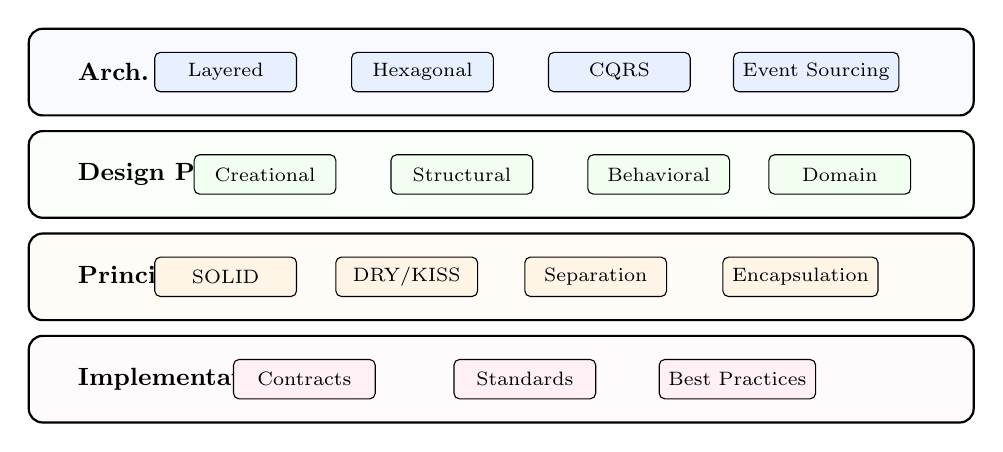
\begin{tikzpicture}[
    node distance=1cm and 1.5cm,
    layer/.style={draw, thick, rounded corners=5pt, minimum width=12cm, minimum height=1.1cm, font=\small},
    element/.style={draw, rounded corners=2pt, minimum width=1.8cm, minimum height=0.5cm, font=\scriptsize},
]
    % Layers
    \node[layer, fill=patterncolor!30] (arch) at (0, 3.5) {};
    \node[font=\small\bfseries, anchor=west] at (-5.5, 3.5) {Arch. Patterns};
    
    \node[layer, fill=decisioncolor!30] (design) at (0, 2.2) {};
    \node[font=\small\bfseries, anchor=west] at (-5.5, 2.2) {Design Patterns};
    
    \node[layer, fill=principlecolor!30] (principles) at (0, 0.9) {};
    \node[font=\small\bfseries, anchor=west] at (-5.5, 0.9) {Principles};
    
    \node[layer, fill=interfacecolor!30] (impl) at (0, -0.4) {};
    \node[font=\small\bfseries, anchor=west] at (-5.5, -0.4) {Implementation};
    
    % Architectural pattern elements
    \node[element, fill=patterncolor] at (-3.5, 3.5) {Layered};
    \node[element, fill=patterncolor] at (-1, 3.5) {Hexagonal};
    \node[element, fill=patterncolor] at (1.5, 3.5) {CQRS};
    \node[element, fill=patterncolor] at (4, 3.5) {Event Sourcing};
    
    % Design pattern elements
    \node[element, fill=decisioncolor] at (-3, 2.2) {Creational};
    \node[element, fill=decisioncolor] at (-0.5, 2.2) {Structural};
    \node[element, fill=decisioncolor] at (2, 2.2) {Behavioral};
    \node[element, fill=decisioncolor] at (4.3, 2.2) {Domain};
    
    % Principle elements
    \node[element, fill=principlecolor] at (-3.5, 0.9) {SOLID};
    \node[element, fill=principlecolor] at (-1.2, 0.9) {DRY/KISS};
    \node[element, fill=principlecolor] at (1.2, 0.9) {Separation};
    \node[element, fill=principlecolor] at (3.8, 0.9) {Encapsulation};
    
    % Implementation elements
    \node[element, fill=interfacecolor] at (-2.5, -0.4) {Contracts};
    \node[element, fill=interfacecolor] at (0.3, -0.4) {Standards};
    \node[element, fill=interfacecolor] at (3, -0.4) {Best Practices};
    
\end{tikzpicture}
\caption{Design Architecture Layers}
\end{figure}

% =============================================================================
% SECTION: CONCERNS
% =============================================================================
\section{Concerns}

This section enumerates the design concerns that the Designer's View is designed to address.

\subsection{Primary Concerns}

\begin{enumerate}[label=\textbf{C\arabic*:}, leftmargin=2.5em]
    \item \textbf{Architectural Pattern Selection}
    \begin{itemize}[nosep]
        \item What architectural patterns structure the system?
        \item Why were these patterns chosen?
        \item How do patterns interact?
        \item What are the pattern boundaries?
        \item What variations are applied?
    \end{itemize}
    
    \item \textbf{Design Pattern Application}
    \begin{itemize}[nosep]
        \item Which design patterns should be used where?
        \item How are patterns implemented in this context?
        \item What adaptations are needed?
        \item How do patterns compose?
        \item What anti-patterns should be avoided?
    \end{itemize}
    
    \item \textbf{Design Principles Adherence}
    \begin{itemize}[nosep]
        \item What principles guide design decisions?
        \item How are SOLID principles applied?
        \item Where are exceptions allowed?
        \item How is principle adherence verified?
        \item What trade-offs exist between principles?
    \end{itemize}
    
    \item \textbf{Interface Design}
    \begin{itemize}[nosep]
        \item How are interfaces defined?
        \item What contracts must implementations honor?
        \item How is versioning handled?
        \item What documentation is required?
        \item How are breaking changes managed?
    \end{itemize}
    
    \item \textbf{Design Decision Documentation}
    \begin{itemize}[nosep]
        \item What key decisions were made?
        \item What alternatives were considered?
        \item What is the rationale for each decision?
        \item What trade-offs were accepted?
        \item When should decisions be revisited?
    \end{itemize}
    
    \item \textbf{Quality Attribute Tactics}
    \begin{itemize}[nosep]
        \item What tactics achieve performance goals?
        \item How is reliability ensured?
        \item What security patterns are used?
        \item How is maintainability supported?
        \item What testability considerations exist?
    \end{itemize}
    
    \item \textbf{Error Handling Strategy}
    \begin{itemize}[nosep]
        \item How are errors represented?
        \item What exception hierarchy exists?
        \item How are errors propagated?
        \item What recovery strategies exist?
        \item How are errors logged and monitored?
    \end{itemize}
    
    \item \textbf{Cross-Cutting Concerns}
    \begin{itemize}[nosep]
        \item How is logging implemented?
        \item How is authentication/authorization handled?
        \item How is caching managed?
        \item How is validation performed?
        \item How are transactions managed?
    \end{itemize}
    
    \item \textbf{Code Organization}
    \begin{itemize}[nosep]
        \item How is code structured within modules?
        \item What naming conventions apply?
        \item How are dependencies managed?
        \item What layering exists within components?
        \item How is code reuse achieved?
    \end{itemize}
    
    \item \textbf{Testing Strategy}
    \begin{itemize}[nosep]
        \item How is testability designed in?
        \item What testing patterns are used?
        \item How are dependencies mocked?
        \item What test coverage is expected?
        \item How are integration tests structured?
    \end{itemize}
\end{enumerate}

\subsection{Concern-Quality Attribute Mapping}

\begin{table}[H]
\centering
\caption{Concern to Quality Attribute Mapping}
\small
\begin{tabular}{@{}L{2.8cm}C{1cm}C{1cm}C{1cm}C{1cm}C{1cm}C{1cm}C{1cm}C{1cm}@{}}
\toprule
\textbf{Concern} & \rotatebox{60}{\textbf{Maintain.}} & \rotatebox{60}{\textbf{Testabil.}} & \rotatebox{60}{\textbf{Perform.}} & \rotatebox{60}{\textbf{Security}} & \rotatebox{60}{\textbf{Reliabil.}} & \rotatebox{60}{\textbf{Reusabil.}} & \rotatebox{60}{\textbf{Flextic.}} & \rotatebox{60}{\textbf{Underst.}} \\
\midrule
Arch. Patterns & $\bullet$ & $\circ$ & $\circ$ & $\circ$ & $\circ$ & $\circ$ & $\bullet$ & $\bullet$ \\
Design Patterns & $\bullet$ & $\bullet$ & $\circ$ & $\circ$ & $\circ$ & $\bullet$ & $\bullet$ & $\circ$ \\
Principles & $\bullet$ & $\bullet$ & -- & -- & $\circ$ & $\bullet$ & $\bullet$ & $\bullet$ \\
Interfaces & $\bullet$ & $\bullet$ & $\circ$ & $\circ$ & $\circ$ & $\bullet$ & $\bullet$ & $\circ$ \\
Decisions & $\circ$ & $\circ$ & $\circ$ & $\circ$ & $\circ$ & $\circ$ & $\circ$ & $\bullet$ \\
QA Tactics & $\circ$ & $\circ$ & $\bullet$ & $\bullet$ & $\bullet$ & -- & $\circ$ & -- \\
Error Handling & $\circ$ & $\circ$ & $\circ$ & $\circ$ & $\bullet$ & $\circ$ & $\circ$ & $\circ$ \\
Cross-Cutting & $\bullet$ & $\circ$ & $\circ$ & $\bullet$ & $\circ$ & $\bullet$ & $\circ$ & $\circ$ \\
Code Org. & $\bullet$ & $\bullet$ & -- & -- & -- & $\bullet$ & $\circ$ & $\bullet$ \\
Testing & $\circ$ & $\bullet$ & -- & $\circ$ & $\bullet$ & $\circ$ & $\circ$ & $\circ$ \\
\bottomrule
\multicolumn{9}{l}{\footnotesize $\bullet$ = Primary impact, $\circ$ = Secondary impact, -- = Minimal impact}
\end{tabular}
\end{table}

% =============================================================================
% SECTION: ANTI-CONCERNS
% =============================================================================
\section{Anti-Concerns}

Understanding what the Designer's View is \emph{not} appropriate for helps stakeholders avoid misapplying this viewpoint.

\subsection{Out of Scope Topics}

\begin{enumerate}[label=\textbf{AC\arabic*:}, leftmargin=2.5em]
    \item \textbf{Business Requirements}
    \begin{itemize}[nosep]
        \item Functional requirements specification
        \item User stories and acceptance criteria
        \item Business rules definition
        \item Use case descriptions
        \item Feature prioritization
    \end{itemize}
    
    \item \textbf{Deployment and Operations}
    \begin{itemize}[nosep]
        \item Infrastructure configuration
        \item Container orchestration
        \item Deployment procedures
        \item Monitoring setup
        \item Incident management
    \end{itemize}
    
    \item \textbf{Project Management}
    \begin{itemize}[nosep]
        \item Team organization
        \item Sprint planning
        \item Resource allocation
        \item Timeline management
        \item Risk management
    \end{itemize}
    
    \item \textbf{High-Level Architecture}
    \begin{itemize}[nosep]
        \item System context
        \item External integrations
        \item Deployment topology
        \item Technology selection rationale
        \item Capacity planning
    \end{itemize}
    
    \item \textbf{Detailed Algorithm Implementation}
    \begin{itemize}[nosep]
        \item Specific algorithm code
        \item Mathematical formulas
        \item Data structure implementations
        \item Performance optimizations
        \item Platform-specific code
    \end{itemize}
\end{enumerate}

\begin{warningbox}[Common Misapplications]
Avoid using the Designer's View for:

\begin{itemize}[nosep]
    \item Defining what the system should do (use Requirements)
    \item High-level system structure (use Logical/C\&C Views)
    \item Deployment and infrastructure (use Deployment View)
    \item Team and work organization (use Planner's View)
    \item Detailed code documentation (use code comments/API docs)
\end{itemize}
\end{warningbox}

% =============================================================================
% SECTION: TYPICAL STAKEHOLDERS
% =============================================================================
\section{Typical Stakeholders}

The Designer's View serves stakeholders involved in detailed system design and implementation.

\subsection{Primary Stakeholders}

\begin{table}[H]
\centering
\caption{Primary Stakeholder Analysis}
\small
\begin{tabular}{@{}L{2.6cm}L{3.6cm}L{7cm}@{}}
\toprule
\textbf{Stakeholder} & \textbf{Role Description} & \textbf{Primary Interests} \\
\midrule
Software Designers & Create detailed designs & Pattern selection, design decisions, quality tactics \\
\addlinespace
Senior Developers & Implement complex features & Implementation guidance, patterns, best practices \\
\addlinespace
Tech Leads & Guide team implementation & Standards, consistency, design review criteria \\
\addlinespace
Software Architects & Define design standards & Pattern catalog, principles, decision framework \\
\addlinespace
Code Reviewers & Evaluate implementations & Design compliance, pattern usage, principle adherence \\
\addlinespace
QA Engineers & Design test strategies & Testability patterns, test design, coverage guidance \\
\bottomrule
\end{tabular}
\end{table}

\subsection{Secondary Stakeholders}

\begin{table}[H]
\centering
\caption{Secondary Stakeholder Analysis}
\small
\begin{tabular}{@{}L{2.6cm}L{3.6cm}L{7cm}@{}}
\toprule
\textbf{Stakeholder} & \textbf{Role Description} & \textbf{Primary Interests} \\
\midrule
Junior Developers & Learn and implement & Learning patterns, understanding decisions \\
\addlinespace
DevOps Engineers & Automate and deploy & Build integration, deployment patterns \\
\addlinespace
Security Engineers & Ensure security & Security patterns, secure coding practices \\
\addlinespace
Performance Eng. & Optimize performance & Performance patterns, optimization techniques \\
\addlinespace
Technical Writers & Document system & Design documentation, API specifications \\
\addlinespace
New Team Members & Onboard to project & Understanding design philosophy, conventions \\
\bottomrule
\end{tabular}
\end{table}

\subsection{Stakeholder Concern Matrix}

\begin{table}[H]
\centering
\caption{Stakeholder-Concern Responsibility Matrix}
\footnotesize
\begin{tabular}{@{}L{2cm}C{0.8cm}C{0.8cm}C{0.8cm}C{0.8cm}C{0.8cm}C{0.8cm}C{0.8cm}C{0.8cm}C{0.8cm}C{0.8cm}@{}}
\toprule
& \rotatebox{60}{\textbf{Arch Pat.}} & \rotatebox{60}{\textbf{Design Pat.}} & \rotatebox{60}{\textbf{Principles}} & \rotatebox{60}{\textbf{Interfaces}} & \rotatebox{60}{\textbf{Decisions}} & \rotatebox{60}{\textbf{QA Tactics}} & \rotatebox{60}{\textbf{Errors}} & \rotatebox{60}{\textbf{Cross-Cut}} & \rotatebox{60}{\textbf{Code Org}} & \rotatebox{60}{\textbf{Testing}} \\
\midrule
Architect & R & A & R & A & A & R & A & R & A & C \\
Designer & C & R & R & R & R & R & R & R & R & R \\
Sr. Developer & I & R & R & R & C & C & R & R & R & R \\
Tech Lead & C & R & R & R & R & C & R & R & R & R \\
Reviewer & I & C & C & C & I & I & C & C & C & C \\
QA Engineer & I & I & I & C & I & C & C & I & I & R \\
\bottomrule
\multicolumn{11}{l}{\footnotesize R = Responsible, A = Accountable, C = Consulted, I = Informed}
\end{tabular}
\end{table}

% =============================================================================
% SECTION: MODEL TYPES
% =============================================================================
\section{Model Types}

The Designer's View employs several complementary model types to capture design knowledge.

\subsection{Model Type Catalog}

\begin{enumerate}[label=\textbf{MT\arabic*:}, leftmargin=2.5em]
    \item \textbf{Pattern Catalog}
    \begin{itemize}[nosep]
        \item \textit{Purpose:} Document applicable patterns
        \item \textit{Primary Elements:} Patterns, contexts, applications
        \item \textit{Key Relationships:} Applies-to, composes-with
        \item \textit{Typical Notation:} Pattern templates, class diagrams
    \end{itemize}
    
    \item \textbf{Architecture Decision Records (ADRs)}
    \begin{itemize}[nosep]
        \item \textit{Purpose:} Document significant decisions
        \item \textit{Primary Elements:} Decisions, context, consequences
        \item \textit{Key Relationships:} Supersedes, relates-to
        \item \textit{Typical Notation:} ADR templates (Markdown)
    \end{itemize}
    
    \item \textbf{Interface Specifications}
    \begin{itemize}[nosep]
        \item \textit{Purpose:} Define contracts between components
        \item \textit{Primary Elements:} Interfaces, methods, types
        \item \textit{Key Relationships:} Implements, extends
        \item \textit{Typical Notation:} Interface definitions, OpenAPI
    \end{itemize}
    
    \item \textbf{Class/Structure Diagrams}
    \begin{itemize}[nosep]
        \item \textit{Purpose:} Show detailed class relationships
        \item \textit{Primary Elements:} Classes, relationships, methods
        \item \textit{Key Relationships:} Inherits, composes, uses
        \item \textit{Typical Notation:} UML class diagrams
    \end{itemize}
    
    \item \textbf{Sequence Diagrams}
    \begin{itemize}[nosep]
        \item \textit{Purpose:} Show interaction flows
        \item \textit{Primary Elements:} Objects, messages, lifelines
        \item \textit{Key Relationships:} Calls, returns
        \item \textit{Typical Notation:} UML sequence diagrams
    \end{itemize}
    
    \item \textbf{State Diagrams}
    \begin{itemize}[nosep]
        \item \textit{Purpose:} Model object state behavior
        \item \textit{Primary Elements:} States, transitions, events
        \item \textit{Key Relationships:} Transitions-to, triggers
        \item \textit{Typical Notation:} UML state machine diagrams
    \end{itemize}
    
    \item \textbf{Coding Standards Document}
    \begin{itemize}[nosep]
        \item \textit{Purpose:} Define coding conventions
        \item \textit{Primary Elements:} Rules, examples, rationale
        \item \textit{Key Relationships:} Applies-to, overrides
        \item \textit{Typical Notation:} Style guides, linter configs
    \end{itemize}
    
    \item \textbf{Error Handling Guide}
    \begin{itemize}[nosep]
        \item \textit{Purpose:} Define error handling strategy
        \item \textit{Primary Elements:} Error types, handlers, policies
        \item \textit{Key Relationships:} Handles, propagates
        \item \textit{Typical Notation:} Exception hierarchies, flow diagrams
    \end{itemize}
    
    \item \textbf{Quality Attribute Tactics Catalog}
    \begin{itemize}[nosep]
        \item \textit{Purpose:} Document tactics for quality attributes
        \item \textit{Primary Elements:} Attributes, tactics, implementations
        \item \textit{Key Relationships:} Achieves, supports
        \item \textit{Typical Notation:} Tactic tables, decision trees
    \end{itemize}
\end{enumerate}

\subsection{Model Type Relationships}

\begin{figure}[H]
\centering
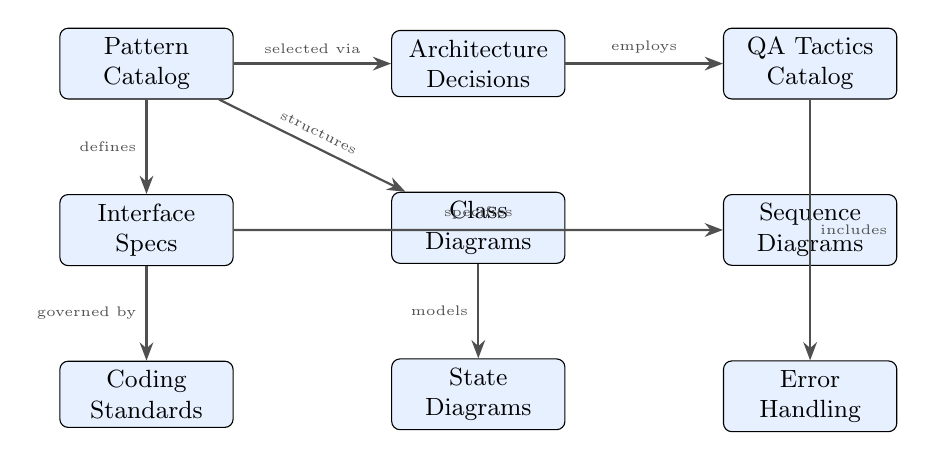
\begin{tikzpicture}[
    node distance=1.2cm and 2cm,
    model/.style={draw, fill=patterncolor, rounded corners=3pt, minimum width=2.2cm, minimum height=0.7cm, font=\small, align=center},
    arrow/.style={-{Stealth}, thick, darkgray}
]
    % Nodes - top row
    \node[model] (patterns) {Pattern\\Catalog};
    \node[model, right=2cm of patterns] (adrs) {Architecture\\Decisions};
    \node[model, right=2cm of adrs] (tactics) {QA Tactics\\Catalog};
    
    % Nodes - middle row
    \node[model, below=1.2cm of patterns] (interfaces) {Interface\\Specs};
    \node[model, below=1.2cm of adrs] (class) {Class\\Diagrams};
    \node[model, below=1.2cm of tactics] (sequence) {Sequence\\Diagrams};
    
    % Nodes - bottom row
    \node[model, below=1.2cm of interfaces] (standards) {Coding\\Standards};
    \node[model, below=1.2cm of class] (state) {State\\Diagrams};
    \node[model, below=1.2cm of sequence] (errors) {Error\\Handling};
    
    % Arrows
    \draw[arrow] (patterns) -- (adrs) node[midway, above, font=\tiny] {selected via};
    \draw[arrow] (adrs) -- (tactics) node[midway, above, font=\tiny] {employs};
    \draw[arrow] (patterns) -- (interfaces) node[midway, left, font=\tiny] {defines};
    \draw[arrow] (patterns) -- (class) node[midway, above, sloped, font=\tiny] {structures};
    \draw[arrow] (interfaces) -- (sequence) node[midway, above, font=\tiny] {specifies};
    \draw[arrow] (class) -- (state) node[midway, left, font=\tiny] {models};
    \draw[arrow] (tactics) -- (errors) node[midway, right, font=\tiny] {includes};
    \draw[arrow] (interfaces) -- (standards) node[midway, left, font=\tiny] {governed by};
\end{tikzpicture}
\caption{Model Type Dependency Relationships}
\end{figure}

% =============================================================================
% SECTION: MODEL LANGUAGES
% =============================================================================
\section{Model Languages}

For each model type, specific languages, notations, and techniques are prescribed.

\subsection{Design Element Notation}

\begin{figure}[H]
\centering
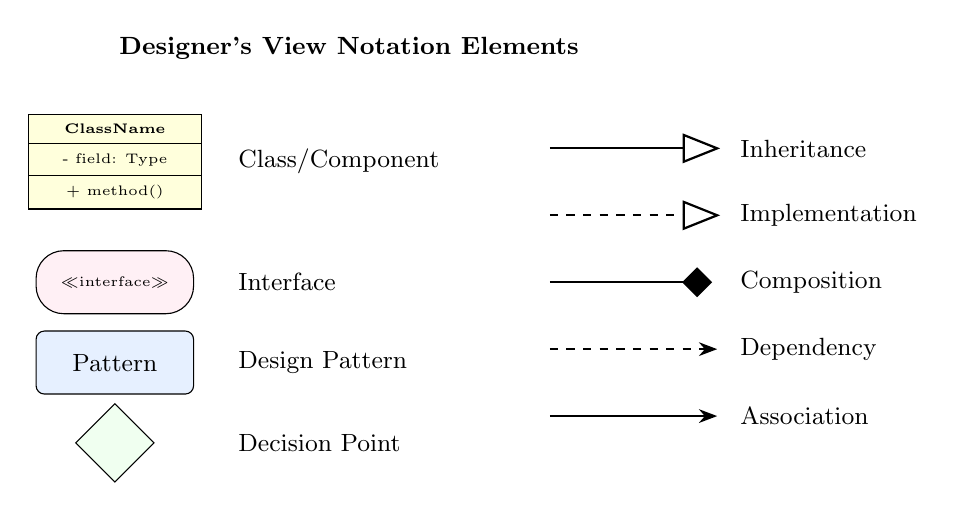
\begin{tikzpicture}[scale=0.85]
    % Legend title
    \node[font=\small\bfseries] at (0, 5) {Designer's View Notation Elements};
    
    % Class
    \node[draw, fill=classcolor, rectangle split, rectangle split parts=3, minimum width=2.2cm, font=\tiny] at (-3.5, 3.3) {
        \textbf{ClassName}
        \nodepart{second}
        - field: Type
        \nodepart{third}
        + method()
    };
    \node[right, font=\small] at (-1.8, 3.3) {Class/Component};
    
    % Interface
    \node[draw, fill=interfacecolor, rounded corners=10pt, minimum width=2cm, minimum height=0.8cm] at (-3.5, 1.5) {};
    \node[font=\tiny] at (-3.5, 1.5) {$\ll$interface$\gg$};
    \node[right, font=\small] at (-1.8, 1.5) {Interface};
    
    % Pattern
    \node[draw, fill=patterncolor, rounded corners=3pt, minimum width=2cm, minimum height=0.8cm] at (-3.5, 0.3) {};
    \node[font=\small] at (-3.5, 0.3) {Pattern};
    \node[right, font=\small] at (-1.8, 0.3) {Design Pattern};
    
    % Decision
    \node[draw, fill=decisioncolor, diamond, minimum size=1cm] at (-3.5, -0.9) {};
    \node[right, font=\small] at (-1.8, -0.9) {Decision Point};
    
    % Inheritance
    \draw[thick] (3, 3.5) -- (5, 3.5);
    \draw[thick, fill=white] (5, 3.3) -- (5, 3.7) -- (5.5, 3.5) -- cycle;
    \node[right, font=\small] at (5.7, 3.5) {Inheritance};
    
    % Implementation
    \draw[thick, dashed] (3, 2.5) -- (5, 2.5);
    \draw[thick, fill=white] (5, 2.3) -- (5, 2.7) -- (5.5, 2.5) -- cycle;
    \node[right, font=\small] at (5.7, 2.5) {Implementation};
    
    % Composition
    \draw[thick] (3, 1.5) -- (5, 1.5);
    \draw[thick, fill=black] (5, 1.5) -- (5.2, 1.7) -- (5.4, 1.5) -- (5.2, 1.3) -- cycle;
    \node[right, font=\small] at (5.7, 1.5) {Composition};
    
    % Dependency
    \draw[-{Stealth}, thick, dashed] (3, 0.5) -- (5.5, 0.5);
    \node[right, font=\small] at (5.7, 0.5) {Dependency};
    
    % Association
    \draw[-{Stealth}, thick] (3, -0.5) -- (5.5, -0.5);
    \node[right, font=\small] at (5.7, -0.5) {Association};
    
\end{tikzpicture}
\caption{Designer's View Notation Legend}
\end{figure}

\subsection{SOLID Principles}

\begin{table}[H]
\centering
\caption{SOLID Design Principles}
\small
\begin{tabular}{@{}L{1cm}L{3.5cm}L{8cm}@{}}
\toprule
\textbf{} & \textbf{Principle} & \textbf{Description} \\
\midrule
S & Single Responsibility & A class should have only one reason to change \\
\addlinespace
O & Open/Closed & Open for extension, closed for modification \\
\addlinespace
L & Liskov Substitution & Subtypes must be substitutable for base types \\
\addlinespace
I & Interface Segregation & Many specific interfaces over one general interface \\
\addlinespace
D & Dependency Inversion & Depend on abstractions, not concretions \\
\bottomrule
\end{tabular}
\end{table}

\subsection{Design Pattern Categories}

\begin{table}[H]
\centering
\caption{Design Pattern Classification}
\small
\begin{tabular}{@{}L{2.5cm}L{4.5cm}L{5.5cm}@{}}
\toprule
\textbf{Category} & \textbf{Purpose} & \textbf{Key Patterns} \\
\midrule
Creational & Object creation mechanisms & Factory, Abstract Factory, Builder, Singleton, Prototype \\
\addlinespace
Structural & Object composition & Adapter, Bridge, Composite, Decorator, Facade, Proxy \\
\addlinespace
Behavioral & Object interaction & Strategy, Observer, Command, State, Chain of Responsibility \\
\addlinespace
Domain & Domain model patterns & Repository, Aggregate, Entity, Value Object, Domain Event \\
\addlinespace
Architectural & System structure & Layered, Hexagonal, CQRS, Event Sourcing, Microservices \\
\addlinespace
Integration & System integration & API Gateway, Circuit Breaker, Retry, Bulkhead, Saga \\
\bottomrule
\end{tabular}
\end{table}

\subsection{Architecture Decision Record Template}

\begin{definitionbox}[ADR Template]
\textbf{Title:} ADR-NNN: [Decision Title]

\textbf{Status:} [Proposed | Accepted | Deprecated | Superseded]

\textbf{Context:} What is the issue that we're seeing that is motivating this decision or change?

\textbf{Decision:} What is the change that we're proposing and/or doing?

\textbf{Consequences:} What becomes easier or more difficult to do because of this change?

\textbf{Alternatives Considered:}
\begin{itemize}[nosep]
    \item Alternative 1: Description and why not chosen
    \item Alternative 2: Description and why not chosen
\end{itemize}
\end{definitionbox}

\subsection{Tabular Specifications}

\subsubsection{Pattern Application Table}

\begin{table}[H]
\centering
\caption{Example Pattern Application Matrix}
\small
\begin{tabular}{@{}L{2.5cm}L{2.5cm}L{3.5cm}L{3.5cm}@{}}
\toprule
\textbf{Pattern} & \textbf{Category} & \textbf{Applied To} & \textbf{Purpose} \\
\midrule
Repository & Domain & Data access layer & Abstract persistence operations \\
\addlinespace
Factory & Creational & Service creation & Centralize object instantiation \\
\addlinespace
Strategy & Behavioral & Payment processing & Swap payment providers \\
\addlinespace
Observer & Behavioral & Event system & Decouple event producers/consumers \\
\addlinespace
Decorator & Structural & Logging, caching & Add cross-cutting concerns \\
\addlinespace
Adapter & Structural & External APIs & Normalize external interfaces \\
\bottomrule
\end{tabular}
\end{table}

\subsubsection{Quality Attribute Tactics Table}

\begin{table}[H]
\centering
\caption{Example Quality Attribute Tactics}
\small
\begin{tabular}{@{}L{2cm}L{2.5cm}L{4cm}L{3.5cm}@{}}
\toprule
\textbf{Attribute} & \textbf{Tactic} & \textbf{Implementation} & \textbf{Trade-off} \\
\midrule
Performance & Caching & Redis for session, API responses & Memory cost, staleness \\
\addlinespace
Performance & Connection Pool & HikariCP, 20-50 connections & Resource usage \\
\addlinespace
Reliability & Circuit Breaker & Resilience4j, 50\% threshold & Temporary unavailability \\
\addlinespace
Reliability & Retry & Exponential backoff, 3 retries & Increased latency \\
\addlinespace
Security & Input Validation & Schema validation at boundaries & Processing overhead \\
\addlinespace
Testability & Dependency Injection & Constructor injection & Code complexity \\
\bottomrule
\end{tabular}
\end{table}

% =============================================================================
% SECTION: VIEWPOINT METAMODELS
% =============================================================================
\section{Viewpoint Metamodels}

This section defines the conceptual metamodel underlying the Designer's View.

\subsection{Core Metamodel}

\begin{figure}[H]
\centering
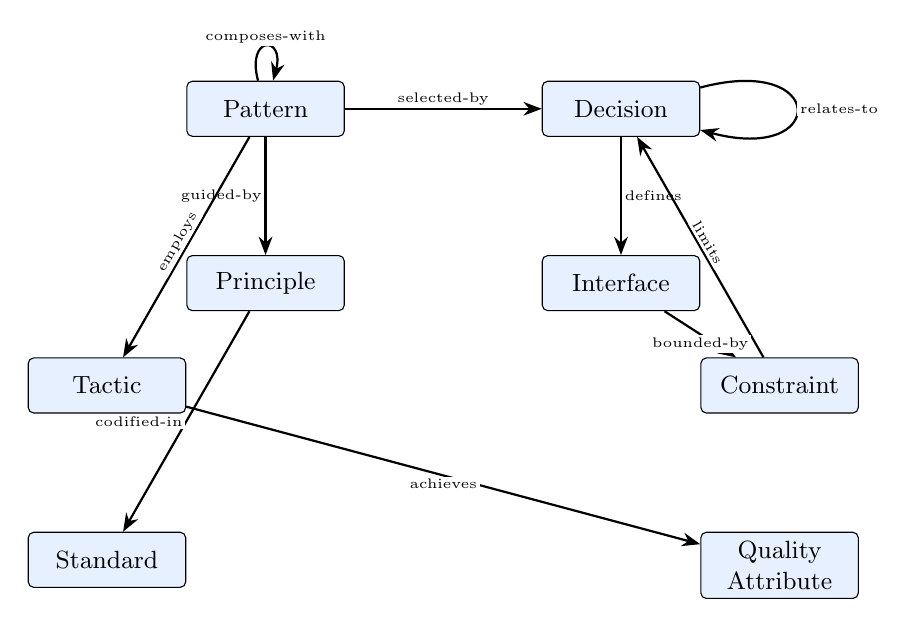
\begin{tikzpicture}[
    node distance=1.3cm and 2cm,
    entity/.style={draw, fill=patterncolor, rounded corners=2pt, minimum width=2cm, minimum height=0.7cm, font=\small, align=center},
    arrow/.style={-{Stealth}, thick},
    label/.style={font=\tiny, fill=white, inner sep=1pt}
]
    % Main entities
    \node[entity] (pattern) {Pattern};
    \node[entity, right=2.5cm of pattern] (decision) {Decision};
    \node[entity, below=1.5cm of pattern] (principle) {Principle};
    \node[entity, below=1.5cm of decision] (interface) {Interface};
    \node[entity, below left=2.8cm and 0cm of pattern] (tactic) {Tactic};
    \node[entity, below right=2.8cm and 0cm of decision] (constraint) {Constraint};
    \node[entity, below=1.5cm of tactic] (standard) {Standard};
    \node[entity, below=1.5cm of constraint] (qa) {Quality\\Attribute};
    
    % Relationships
    \draw[arrow] (pattern) -- (decision) node[label, midway, above] {selected-by};
    \draw[arrow] (pattern) -- (principle) node[label, midway, left] {guided-by};
    \draw[arrow] (decision) -- (interface) node[label, midway, right] {defines};
    \draw[arrow] (principle) -- (standard) node[label, midway, left] {codified-in};
    \draw[arrow] (tactic) -- (qa) node[label, midway, below] {achieves};
    \draw[arrow] (constraint) -- (decision) node[label, midway, above, sloped] {limits};
    \draw[arrow] (pattern) -- (tactic) node[label, midway, above, sloped] {employs};
    \draw[arrow] (interface) -- (constraint) node[label, midway, below] {bounded-by};
    
    % Self-reference
    \draw[arrow] (pattern) to[loop above] node[label, above] {composes-with} (pattern);
    \draw[arrow] (decision) to[loop right] node[label, right] {relates-to} (decision);
\end{tikzpicture}
\caption{Designer's View Core Metamodel}
\end{figure}

\subsection{Entity Definitions}

\begin{definitionbox}[Entity: Pattern]
\textbf{Definition:} A reusable solution to a commonly occurring design problem within a given context.

\textbf{Attributes:}
\begin{itemize}[nosep]
    \item \texttt{patternId}: Unique identifier
    \item \texttt{name}: Pattern name
    \item \texttt{category}: Pattern category (creational, structural, behavioral, etc.)
    \item \texttt{intent}: What the pattern does
    \item \texttt{problem}: Problem the pattern solves
    \item \texttt{solution}: How the pattern solves the problem
    \item \texttt{structure}: Structural diagram
    \item \texttt{participants}: Key classes/interfaces
    \item \texttt{consequences}: Trade-offs and results
    \item \texttt{applicability}: When to use
    \item \texttt{relatedPatterns}: Related patterns
\end{itemize}

\textbf{Constraints:}
\begin{itemize}[nosep]
    \item Pattern should solve a recurring problem
    \item Trade-offs should be documented
    \item Applicability criteria should be clear
\end{itemize}
\end{definitionbox}

\begin{definitionbox}[Entity: Decision]
\textbf{Definition:} A significant technical choice that affects system design with documented rationale and consequences.

\textbf{Attributes:}
\begin{itemize}[nosep]
    \item \texttt{decisionId}: Unique identifier (ADR number)
    \item \texttt{title}: Decision title
    \item \texttt{status}: Current status (proposed, accepted, deprecated, superseded)
    \item \texttt{context}: Circumstances driving the decision
    \item \texttt{decision}: The choice made
    \item \texttt{rationale}: Why this choice was made
    \item \texttt{alternatives}: Other options considered
    \item \texttt{consequences}: Positive and negative outcomes
    \item \texttt{date}: When decision was made
    \item \texttt{deciders}: Who made the decision
    \item \texttt{supersedes}: Previous decision replaced
\end{itemize}

\textbf{Constraints:}
\begin{itemize}[nosep]
    \item Significant decisions should be documented
    \item Alternatives should be captured
    \item Consequences should include trade-offs
\end{itemize}
\end{definitionbox}

\begin{definitionbox}[Entity: Principle]
\textbf{Definition:} A fundamental guideline that directs design decisions and promotes desired qualities.

\textbf{Attributes:}
\begin{itemize}[nosep]
    \item \texttt{principleId}: Unique identifier
    \item \texttt{name}: Principle name
    \item \texttt{statement}: Concise principle statement
    \item \texttt{rationale}: Why this principle matters
    \item \texttt{implications}: What following this means
    \item \texttt{examples}: Examples of application
    \item \texttt{counterExamples}: Examples of violation
    \item \texttt{exceptions}: When exceptions are allowed
    \item \texttt{qualityAttributes}: Qualities supported
\end{itemize}

\textbf{Constraints:}
\begin{itemize}[nosep]
    \item Principles should be actionable
    \item Exceptions should be documented
    \item Conflicts between principles should be resolved
\end{itemize}
\end{definitionbox}

\begin{definitionbox}[Entity: Interface]
\textbf{Definition:} A contract defining the operations, data types, and behaviors that an implementation must provide.

\textbf{Attributes:}
\begin{itemize}[nosep]
    \item \texttt{interfaceId}: Unique identifier
    \item \texttt{name}: Interface name
    \item \texttt{description}: Interface purpose
    \item \texttt{version}: Interface version
    \item \texttt{operations}: List of operations
    \item \texttt{types}: Data types used
    \item \texttt{preconditions}: Required state before calls
    \item \texttt{postconditions}: Guaranteed state after calls
    \item \texttt{invariants}: Always-true conditions
    \item \texttt{exceptions}: Possible exceptions
    \item \texttt{qualityOfService}: Performance/reliability requirements
\end{itemize}

\textbf{Constraints:}
\begin{itemize}[nosep]
    \item Interfaces should be stable
    \item Breaking changes require versioning
    \item Contracts should be complete
\end{itemize}
\end{definitionbox}

\begin{definitionbox}[Entity: Tactic]
\textbf{Definition:} A specific design technique used to achieve or enhance a particular quality attribute.

\textbf{Attributes:}
\begin{itemize}[nosep]
    \item \texttt{tacticId}: Unique identifier
    \item \texttt{name}: Tactic name
    \item \texttt{qualityAttribute}: Target quality attribute
    \item \texttt{description}: How the tactic works
    \item \texttt{implementation}: How to implement
    \item \texttt{tradeoffs}: Quality trade-offs
    \item \texttt{applicability}: When to use
    \item \texttt{examples}: Implementation examples
    \item \texttt{relatedPatterns}: Patterns that employ this tactic
\end{itemize}

\textbf{Constraints:}
\begin{itemize}[nosep]
    \item Tactics should target specific qualities
    \item Trade-offs should be understood
    \item Implementation should be practical
\end{itemize}
\end{definitionbox}

\begin{definitionbox}[Entity: Constraint]
\textbf{Definition:} A limitation or restriction that bounds design choices.

\textbf{Attributes:}
\begin{itemize}[nosep]
    \item \texttt{constraintId}: Unique identifier
    \item \texttt{name}: Constraint name
    \item \texttt{description}: Constraint description
    \item \texttt{type}: Constraint type (technical, business, regulatory)
    \item \texttt{source}: Where constraint comes from
    \item \texttt{scope}: What the constraint applies to
    \item \texttt{impact}: How it affects design
    \item \texttt{flexibility}: How negotiable it is
    \item \texttt{verification}: How compliance is verified
\end{itemize}

\textbf{Constraints:}
\begin{itemize}[nosep]
    \item Constraints should be justified
    \item Impact should be understood
    \item Verification should be possible
\end{itemize}
\end{definitionbox}

\begin{definitionbox}[Entity: Standard]
\textbf{Definition:} A codified rule or convention that ensures consistency in implementation.

\textbf{Attributes:}
\begin{itemize}[nosep]
    \item \texttt{standardId}: Unique identifier
    \item \texttt{name}: Standard name
    \item \texttt{category}: Standard category (naming, formatting, architecture)
    \item \texttt{rule}: The specific rule
    \item \texttt{rationale}: Why this standard exists
    \item \texttt{examples}: Good and bad examples
    \item \texttt{enforcement}: How it's enforced (manual, automated)
    \item \texttt{exceptions}: Allowed exceptions
    \item \texttt{scope}: Where it applies
\end{itemize}

\textbf{Constraints:}
\begin{itemize}[nosep]
    \item Standards should be enforceable
    \item Exceptions should be documented
    \item Automated enforcement preferred
\end{itemize}
\end{definitionbox}

\begin{definitionbox}[Entity: Quality Attribute]
\textbf{Definition:} A measurable or testable property that indicates how well the system satisfies stakeholders.

\textbf{Attributes:}
\begin{itemize}[nosep]
    \item \texttt{attributeId}: Unique identifier
    \item \texttt{name}: Attribute name
    \item \texttt{definition}: What the attribute means
    \item \texttt{scenarios}: Quality attribute scenarios
    \item \texttt{measures}: How it's measured
    \item \texttt{targets}: Target values
    \item \texttt{tactics}: Tactics that support it
    \item \texttt{tradeoffs}: Conflicts with other attributes
    \item \texttt{priority}: Relative importance
\end{itemize}

\textbf{Constraints:}
\begin{itemize}[nosep]
    \item Attributes should be measurable
    \item Scenarios should be testable
    \item Trade-offs should be explicit
\end{itemize}
\end{definitionbox}

\subsection{Relationship Definitions}

\begin{table}[H]
\centering
\caption{Metamodel Relationship Definitions}
\small
\begin{tabular}{@{}L{2.3cm}L{1.8cm}L{1.8cm}L{7.5cm}@{}}
\toprule
\textbf{Relationship} & \textbf{Source} & \textbf{Target} & \textbf{Description} \\
\midrule
selected-by & Pattern & Decision & Pattern is chosen through decision \\
\addlinespace
guided-by & Pattern & Principle & Pattern application follows principle \\
\addlinespace
defines & Decision & Interface & Decision specifies interface design \\
\addlinespace
codified-in & Principle & Standard & Principle is formalized as standard \\
\addlinespace
achieves & Tactic & QA & Tactic improves quality attribute \\
\addlinespace
limits & Constraint & Decision & Constraint restricts decision options \\
\addlinespace
employs & Pattern & Tactic & Pattern uses tactic for quality \\
\addlinespace
bounded-by & Interface & Constraint & Interface is limited by constraint \\
\addlinespace
composes & Pattern & Pattern & Patterns combine together \\
\addlinespace
relates-to & Decision & Decision & Decisions are interconnected \\
\bottomrule
\end{tabular}
\end{table}

% =============================================================================
% SECTION: CONFORMING NOTATIONS
% =============================================================================
\section{Conforming Notations}

Several existing notations and methods support Designer's View modeling.

\subsection{UML Diagrams}

UML provides comprehensive notation for detailed design:

\textbf{Class Diagrams:} Classes, interfaces, relationships, attributes, methods.

\textbf{Sequence Diagrams:} Object interactions over time.

\textbf{State Machine Diagrams:} Object lifecycle and state transitions.

\textbf{Conformance Level:} High for structural and behavioral design.

\subsection{Architecture Decision Records}

ADRs document significant design decisions:

\textbf{Elements:} Context, decision, consequences, alternatives.

\textbf{Format:} Lightweight Markdown format (Michael Nygard style).

\textbf{Conformance Level:} High for decision documentation.

\subsection{Pattern Languages}

Pattern documentation follows standard templates:

\textbf{Elements:} Name, context, problem, solution, consequences.

\textbf{Sources:} GoF, POSA, EAA, DDD patterns.

\textbf{Conformance Level:} High for pattern documentation.

\subsection{Notation Comparison}

\begin{table}[H]
\centering
\caption{Design Notation Comparison}
\small
\begin{tabular}{@{}L{2.5cm}C{1cm}C{1cm}C{1cm}C{1cm}C{1cm}C{1cm}@{}}
\toprule
\textbf{Feature} & \rotatebox{60}{\textbf{UML}} & \rotatebox{60}{\textbf{ADR}} & \rotatebox{60}{\textbf{Pattern}} & \rotatebox{60}{\textbf{OpenAPI}} & \rotatebox{60}{\textbf{C4}} & \rotatebox{60}{\textbf{Code}} \\
\midrule
Class structure & $\bullet$ & -- & $\circ$ & -- & $\circ$ & $\bullet$ \\
Interactions & $\bullet$ & -- & $\circ$ & $\circ$ & -- & $\circ$ \\
Decisions & -- & $\bullet$ & $\circ$ & -- & -- & -- \\
Patterns & $\circ$ & $\circ$ & $\bullet$ & -- & -- & $\circ$ \\
Interfaces & $\circ$ & -- & -- & $\bullet$ & -- & $\bullet$ \\
State behavior & $\bullet$ & -- & $\circ$ & -- & -- & $\circ$ \\
Standards & -- & -- & -- & $\circ$ & -- & $\bullet$ \\
\bottomrule
\multicolumn{7}{l}{\footnotesize $\bullet$ = Strong support, $\circ$ = Limited support, -- = Not applicable}
\end{tabular}
\end{table}

% =============================================================================
% SECTION: MODEL CORRESPONDENCE RULES
% =============================================================================
\section{Model Correspondence Rules}

Model correspondence rules define how design elements relate to elements in other views.

\subsection{Development View Correspondence}

\begin{definitionbox}[Correspondence Rule CR-01: Pattern to Module Mapping]
\textbf{Rule:} Design patterns should be implemented within appropriate modules.

\textbf{Formal Expression:}
\begin{center}
$\forall p \in Patterns : \exists M \subseteq Modules : implements(M, p)$
\end{center}

\textbf{Rationale:} Ensures patterns are realized in code structure.

\textbf{Verification:} Code review against pattern specifications.
\end{definitionbox}

\begin{definitionbox}[Correspondence Rule CR-02: Standard to Code Mapping]
\textbf{Rule:} Coding standards should be enforced in all code.

\textbf{Formal Expression:}
\begin{center}
$\forall c \in Code : \forall s \in Standards : complies(c, s)$
\end{center}

\textbf{Rationale:} Ensures consistent code quality.

\textbf{Verification:} Automated linting and code review.
\end{definitionbox}

\subsection{Component-and-Connector View Correspondence}

\begin{definitionbox}[Correspondence Rule CR-03: Interface to Component Mapping]
\textbf{Rule:} Design interfaces should be realized as component interfaces.

\textbf{Formal Expression:}
\begin{center}
$\forall i \in DesignInterfaces : \exists c \in Components : realizes(c, i)$
\end{center}

\textbf{Rationale:} Ensures design contracts are implemented at runtime.

\textbf{Verification:} Interface compliance testing.
\end{definitionbox}

% =============================================================================
% SECTION: OPERATIONS ON VIEWS
% =============================================================================
\section{Operations on Views}

This section defines methods for creating, interpreting, analyzing, and maintaining design views.

\subsection{Creation Methods}

\subsubsection{View Development Process}

\begin{guidancebox}[Step 1: Identify Applicable Patterns]
\begin{enumerate}[nosep]
    \item Analyze quality attribute requirements
    \item Review problem contexts
    \item Select candidate architectural patterns
    \item Select candidate design patterns
    \item Document pattern rationale
\end{enumerate}
\end{guidancebox}

\begin{guidancebox}[Step 2: Document Design Decisions]
\begin{enumerate}[nosep]
    \item Identify significant decisions
    \item Document context and drivers
    \item Evaluate alternatives
    \item Record chosen option with rationale
    \item Document consequences and trade-offs
\end{enumerate}
\end{guidancebox}

\begin{guidancebox}[Step 3: Define Interfaces]
\begin{enumerate}[nosep]
    \item Identify interface boundaries
    \item Define operations and signatures
    \item Specify contracts (pre/post conditions)
    \item Document data types
    \item Define error handling
\end{enumerate}
\end{guidancebox}

\begin{guidancebox}[Step 4: Specify Quality Tactics]
\begin{enumerate}[nosep]
    \item Map quality requirements to attributes
    \item Select appropriate tactics
    \item Document implementation approach
    \item Identify trade-offs
    \item Plan verification approach
\end{enumerate}
\end{guidancebox}

\begin{guidancebox}[Step 5: Create Design Models]
\begin{enumerate}[nosep]
    \item Create class diagrams for key structures
    \item Create sequence diagrams for key flows
    \item Create state diagrams for stateful objects
    \item Document pattern applications
    \item Review for consistency
\end{enumerate}
\end{guidancebox}

\begin{guidancebox}[Step 6: Define Standards]
\begin{enumerate}[nosep]
    \item Define naming conventions
    \item Define formatting rules
    \item Define architectural constraints
    \item Configure automated enforcement
    \item Document exceptions process
\end{enumerate}
\end{guidancebox}

\begin{guidancebox}[Step 7: Validate Design]
\begin{enumerate}[nosep]
    \item Review against requirements
    \item Verify pattern applicability
    \item Check principle adherence
    \item Validate interface completeness
    \item Assess quality attribute support
\end{enumerate}
\end{guidancebox}

\subsubsection{Pattern Selection Process}

\begin{patternbox}[Pattern Selection Criteria]
\textbf{Context Fit:}
\begin{itemize}[nosep]
    \item Does the pattern address our specific problem?
    \item Does our context match the pattern's applicability?
    \item Are the pattern's assumptions valid in our context?
\end{itemize}

\textbf{Quality Attribute Support:}
\begin{itemize}[nosep]
    \item Does it support our quality goals?
    \item Are the trade-offs acceptable?
    \item How does it interact with other patterns?
\end{itemize}

\textbf{Implementation Feasibility:}
\begin{itemize}[nosep]
    \item Can our team implement it correctly?
    \item Does it fit our technology stack?
    \item Is the complexity justified?
\end{itemize}
\end{patternbox}

\subsection{Analysis Methods}

\subsubsection{Design Review Checklist}

\begin{definitionbox}[Design Review Criteria]
\textbf{Pattern Application:}
\begin{itemize}[nosep]
    \item Is the pattern implemented correctly?
    \item Are pattern participants properly defined?
    \item Are pattern constraints respected?
\end{itemize}

\textbf{Principle Adherence:}
\begin{itemize}[nosep]
    \item Does each class have single responsibility?
    \item Are abstractions used appropriately?
    \item Is coupling minimized?
\end{itemize}

\textbf{Interface Quality:}
\begin{itemize}[nosep]
    \item Are contracts complete and clear?
    \item Is the interface minimal but sufficient?
    \item Are error cases handled?
\end{itemize}
\end{definitionbox}

% =============================================================================
% SECTION: EXAMPLES
% =============================================================================
\section{Examples}

\subsection{Example 1: Repository Pattern Implementation}

\begin{figure}[H]
\centering
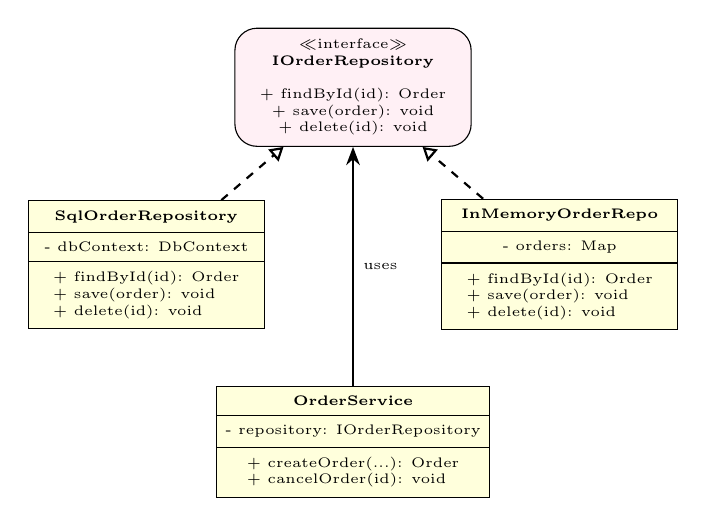
\begin{tikzpicture}[
    class/.style={draw, fill=classcolor, rectangle split, rectangle split parts=3, minimum width=3cm, font=\tiny, align=left},
    interface/.style={draw, fill=interfacecolor, rounded corners=8pt, minimum width=3cm, minimum height=1.5cm, font=\tiny, align=center},
    scale=0.75
]
    % Interface
    \node[interface] (repo) at (0, 3) {
        $\ll$interface$\gg$\\
        \textbf{IOrderRepository}\\
        \\
        + findById(id): Order\\
        + save(order): void\\
        + delete(id): void
    };
    
    % Implementations
    \node[class] (sqlrepo) at (-3.5, 0) {
        \textbf{SqlOrderRepository}
        \nodepart{second}
        - dbContext: DbContext
        \nodepart{third}
        + findById(id): Order\\
        + save(order): void\\
        + delete(id): void
    };
    
    \node[class] (memrepo) at (3.5, 0) {
        \textbf{InMemoryOrderRepo}
        \nodepart{second}
        - orders: Map
        \nodepart{third}
        + findById(id): Order\\
        + save(order): void\\
        + delete(id): void
    };
    
    % Service using repository
    \node[class] (service) at (0, -3) {
        \textbf{OrderService}
        \nodepart{second}
        - repository: IOrderRepository
        \nodepart{third}
        + createOrder(...): Order\\
        + cancelOrder(id): void
    };
    
    % Relationships
    \draw[thick, dashed, -{Triangle[open]}] (sqlrepo) -- (repo);
    \draw[thick, dashed, -{Triangle[open]}] (memrepo) -- (repo);
    \draw[thick, -{Stealth}] (service) -- (repo) node[midway, right, font=\tiny] {uses};
    
\end{tikzpicture}
\caption{Repository Pattern Implementation}
\end{figure}

\textbf{Description:} This class diagram shows the Repository pattern applied to Order persistence. The IOrderRepository interface defines the contract. SqlOrderRepository implements it for production with database persistence. InMemoryOrderRepository provides a test double. OrderService depends only on the interface, enabling easy testing and implementation swapping.

\subsection{Example 2: Architecture Decision Record}

\begin{examplebox}[ADR-005: Use Event Sourcing for Order History]
\textbf{Status:} Accepted

\textbf{Context:} We need to maintain complete order history for audit, customer service, and analytics. Orders go through many state changes and we need to know exactly what happened and when.

\textbf{Decision:} We will use Event Sourcing for the Order aggregate, storing all state changes as a sequence of domain events.

\textbf{Consequences:}
\begin{itemize}[nosep]
    \item \textbf{Positive:} Complete audit trail, temporal queries, replay capability
    \item \textbf{Negative:} Increased complexity, eventual consistency for read models, storage growth
\end{itemize}

\textbf{Alternatives Considered:}
\begin{itemize}[nosep]
    \item \textbf{Audit logging:} Would duplicate data, harder to replay
    \item \textbf{Soft deletes with history table:} Complex triggers, incomplete history
\end{itemize}
\end{examplebox}

\subsection{Example 3: Quality Tactic Implementation}

\begin{table}[H]
\centering
\caption{Circuit Breaker Tactic Configuration}
\small
\begin{tabular}{@{}L{3.5cm}L{3cm}L{5.5cm}@{}}
\toprule
\textbf{Parameter} & \textbf{Value} & \textbf{Rationale} \\
\midrule
Failure Threshold & 50\% & Trip when half of calls fail \\
\addlinespace
Minimum Calls & 10 & Need sample size before tripping \\
\addlinespace
Wait Duration & 30 seconds & Time before attempting recovery \\
\addlinespace
Permitted in Half-Open & 3 calls & Test calls before fully closing \\
\addlinespace
Sliding Window Size & 100 calls & Rolling window for statistics \\
\addlinespace
Fallback Behavior & Return cached data & Graceful degradation \\
\bottomrule
\end{tabular}
\end{table}

% =============================================================================
% SECTION: NOTES
% =============================================================================
\section{Notes}

\subsection{Design Principle Guidelines}

\begin{principlebox}[Design Principle Application]
\begin{itemize}[nosep]
    \item \textbf{Balance Principles:} Principles can conflict; find appropriate balance
    \item \textbf{Context Matters:} Apply principles considering specific context
    \item \textbf{Avoid Dogmatism:} Don't follow principles blindly
    \item \textbf{Document Exceptions:} When violating principles, document why
    \item \textbf{Iterate:} Refactor toward principles as understanding grows
    \item \textbf{Team Agreement:} Ensure team understands and agrees on principles
\end{itemize}
\end{principlebox}

\subsection{Pattern Application Guidelines}

\begin{patternbox}[Effective Pattern Usage]
\begin{itemize}[nosep]
    \item \textbf{Understand Intent:} Know why the pattern exists before using
    \item \textbf{Adapt Appropriately:} Patterns are templates, not rigid rules
    \item \textbf{Avoid Over-Engineering:} Don't use patterns where simple code suffices
    \item \textbf{Combine Carefully:} Understand how patterns interact
    \item \textbf{Name Clearly:} Use pattern names in code for clarity
    \item \textbf{Document Usage:} Explain how pattern is applied in context
\end{itemize}
\end{patternbox}

\subsection{Common Pitfalls}

\begin{warningbox}[Design Anti-Patterns to Avoid]
\begin{enumerate}[nosep]
    \item \textbf{God Class:} Class doing too much, knows too much
    \item \textbf{Spaghetti Code:} Unstructured, tangled control flow
    \item \textbf{Golden Hammer:} Using favorite pattern/tool everywhere
    \item \textbf{Copy-Paste Programming:} Duplicating instead of abstracting
    \item \textbf{Premature Optimization:} Optimizing before measuring
    \item \textbf{Interface Bloat:} Interfaces with too many methods
    \item \textbf{Leaky Abstraction:} Implementation details escaping interface
    \item \textbf{Circular Dependencies:} Modules depending on each other
\end{enumerate}
\end{warningbox}

% =============================================================================
% SECTION: SOURCES
% =============================================================================
\section{Sources}

\subsection{Primary References}

\begin{enumerate}
    \item Gamma, E., Helm, R., Johnson, R., \& Vlissides, J. (1994). \textit{Design Patterns: Elements of Reusable Object-Oriented Software}. Addison-Wesley.
    
    \item Martin, R. C. (2017). \textit{Clean Architecture: A Craftsman's Guide to Software Structure and Design}. Prentice Hall.
    
    \item Fowler, M. (2002). \textit{Patterns of Enterprise Application Architecture}. Addison-Wesley.
    
    \item Evans, E. (2003). \textit{Domain-Driven Design: Tackling Complexity in the Heart of Software}. Addison-Wesley.
    
    \item Bass, L., Clements, P., \& Kazman, R. (2021). \textit{Software Architecture in Practice} (4th ed.). Addison-Wesley.
\end{enumerate}

\subsection{Supplementary References}

\begin{enumerate}[resume]
    \item Freeman, E., \& Robson, E. (2020). \textit{Head First Design Patterns} (2nd ed.). O'Reilly.
    
    \item Nygard, M. (2018). \textit{Release It!} (2nd ed.). Pragmatic Bookshelf.
    
    \item Vernon, V. (2013). \textit{Implementing Domain-Driven Design}. Addison-Wesley.
    
    \item Martin, R. C. (2008). \textit{Clean Code: A Handbook of Agile Software Craftsmanship}. Prentice Hall.
    
    \item Buschmann, F., et al. (1996). \textit{Pattern-Oriented Software Architecture Volume 1}. Wiley.
\end{enumerate}

\subsection{Online Resources}

\begin{itemize}
    \item Refactoring Guru: \url{https://refactoring.guru/design-patterns}
    \item Martin Fowler's Patterns: \url{https://martinfowler.com/}
    \item ADR GitHub Organization: \url{https://adr.github.io/}
    \item Microsoft Design Patterns: \url{https://docs.microsoft.com/azure/architecture/patterns/}
\end{itemize}

% =============================================================================
% APPENDIX
% =============================================================================
\appendix

\section{Designer's View Checklist}

\begin{table}[H]
\centering
\small
\begin{tabular}{@{}L{10cm}C{2cm}@{}}
\toprule
\textbf{Item} & \textbf{Complete?} \\
\midrule
\multicolumn{2}{l}{\textbf{Patterns}} \\
\quad Architectural patterns selected and documented & $\square$ \\
\quad Design patterns identified for key problems & $\square$ \\
\quad Pattern rationale documented & $\square$ \\
\quad Pattern interactions understood & $\square$ \\
\midrule
\multicolumn{2}{l}{\textbf{Decisions}} \\
\quad Significant decisions documented as ADRs & $\square$ \\
\quad Alternatives captured & $\square$ \\
\quad Consequences documented & $\square$ \\
\quad Decision log maintained & $\square$ \\
\midrule
\multicolumn{2}{l}{\textbf{Interfaces}} \\
\quad Key interfaces defined & $\square$ \\
\quad Contracts specified (pre/post conditions) & $\square$ \\
\quad Versioning strategy defined & $\square$ \\
\quad Error handling documented & $\square$ \\
\midrule
\multicolumn{2}{l}{\textbf{Quality}} \\
\quad Quality tactics selected & $\square$ \\
\quad Tactics implementation documented & $\square$ \\
\quad Trade-offs understood & $\square$ \\
\quad Verification approach defined & $\square$ \\
\midrule
\multicolumn{2}{l}{\textbf{Standards}} \\
\quad Coding standards defined & $\square$ \\
\quad Naming conventions documented & $\square$ \\
\quad Automated enforcement configured & $\square$ \\
\quad Team trained on standards & $\square$ \\
\bottomrule
\end{tabular}
\end{table}

\section{Glossary}

\begin{description}[style=nextline, leftmargin=3cm, labelwidth=2.8cm]
    \item[ADR] Architecture Decision Record; documents significant decisions.
    
    \item[Anti-Pattern] A common solution that is counterproductive.
    
    \item[Contract] The specification of obligations and guarantees of an interface.
    
    \item[Design Pattern] A reusable solution to a common design problem.
    
    \item[Invariant] A condition that must always be true.
    
    \item[Postcondition] A condition guaranteed after an operation completes.
    
    \item[Precondition] A condition required before an operation can execute.
    
    \item[Principle] A fundamental guideline directing design decisions.
    
    \item[Quality Attribute] A measurable property indicating system quality.
    
    \item[Refactoring] Improving code structure without changing behavior.
    
    \item[SOLID] Five design principles for maintainable OO code.
    
    \item[Tactic] A specific technique for achieving a quality attribute.
    
    \item[Technical Debt] Cost of rework caused by expedient solutions.
    
    \item[Trade-off] A balance between competing concerns.
\end{description}

% =============================================================================
% END DOCUMENT
% =============================================================================

\end{document}
